%% ----------------------------------------------------------------
%% Evol.tex
%% ---------------------------------------------------------------- 


\chapter{Evolution of Collective Intelligence and Social Network in Web} \label{Chapter:Evolution of Collective Intelligence and Social Network in Web}

In the early 1969 when Internet was invented by ARPANET, it was created as a robust network that allowed military computers to communicate quickly and freely. This network was soon improved when TCP protocol was developed and large data packets could be transmitted through long distance. With the advent of Ethernet, TCP/IP and SMTP protocols and individual personal computers more people were connected to each other, they used Emails to communicate and shared documents to collaborate with each other \cite{segaller1999nerds}.

In the early 1990, development of WWW and HTML at CERN and launch of the first commercial browser, Netscape, Internet had spread to the masses and as of 2011, there are more than 360 million Internet users in the world \cite{internetsats}. The Internet and World Wide Web has become ubiquitous in our everyday life, it has become a vital source of information, means of communication and a channel of self-expression.

The process of globalization has been changed by the WWW, initially only military and academic institutions has the technology to share documents and create mailing lists to communicate, now the web has revolutionized the communication process. People connect to their friends, families and colleagues using different social networking services. They are always in touch with each other using emails, instant messaging services, mobile devices and also using websites like Facebook and Twitter. They interact with complete strangers from all over the world who share same interest as them. The Web 2.0 has made it easier for people to share their personal information and interest with their friends and network, they use different services for different purpose. One person has more than one account to stay connected with the people they know and to share different type of information. WWW has bridged the gap and brought people from different places, socio-economic status and cultures to share and create resources.

The social networking in the web moved forward to create community of like minded people and many tools were used for social collaboration and people contributed to create a collective knowledgebase. This large number of human contribution or crowdsourcing is used to solve many problems that are harder for computers to do and human computation is used to solve many natural language processing, speech recognition and image-processing tasks. The combination of Social Web and human computation provides many opportunities to solve difficult computational problem and create an emergent knowledge to solve problems.

In this section, the report is going to discuss the emergence of Social Web and how the Web has evolved to Web 2.0 that connects all the objects and peoples. In the recent years, the Semantic Web technologies are also incorporated with the web to create a new era of Web 3.0 and it is discussed how these technologies could extend the scope of current social web and social media.

\section{The emergence of Social Web}

The invention of World Wide Web, HTTP and web browsers allowed more people to interact with each other, share documents and create static web page easily, without having a detailed technical and specialized knowledge. Although Tim Berners-Lee had envisioned a read-write web, where the very first browser also worked as an editor, the initial WWW was a read-only web for majority of people. In the early days, the web was mostly a collection of webpages with a phone book like directory to look up individual websites that were connected using hyperlinks.

The passive attitude towards the web changed when the web browsers and search engines made the webpages easily accessible to users and the business world adopted the technology and started using it for e-business. More communication tools like IRC and MS net meeting were developed for organizations to communicate and collaborate. Organization started to have their personal intranet and portals as a collaborative tool and to integrate information on certain topics \cite{stenmark2002information}.

As most of the business world and workplace moved to the digital world, a new phase in the software development emerged, a highly collaborative and alternative model of open source softwares. This was the first wave of crowdsourcing where many programmers and developers came together to build a fully working system and solved problems, Linux software is an important example of this working model.

The web was adopted by more organization, especially the news and entertainment industry and more and more information was put on the web as RSS. People moved from a static personal web page to opinionated blogs and wikis and started the social transformation of the Internet from web of data to web of people. The next section describes this transformation in detail \cite{Albors2008}.


\begin{figure}[!htb]
  \centering
  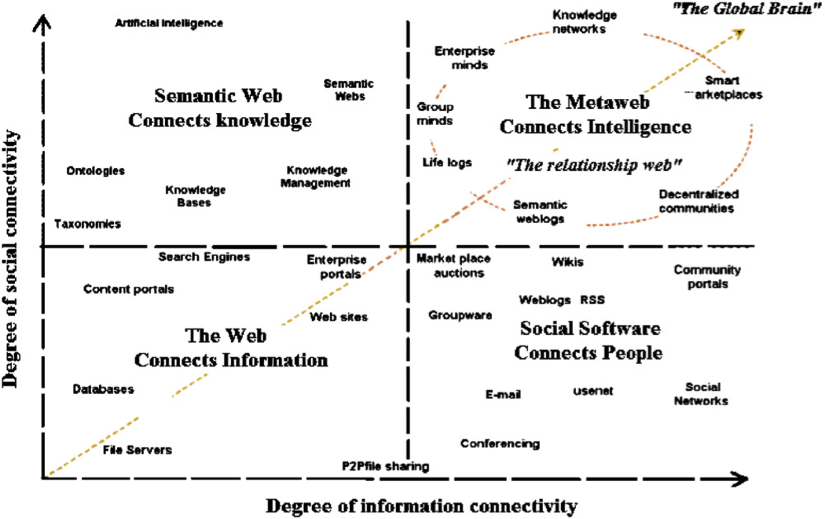
\includegraphics[width=15cm]{bernard.png}
  \caption{A taxonomy for collaboration alternatives \cite{Albors2008}.}
  \label{Figure:figex2c}
\end{figure}

\section{Web 2.0 and Social Media}

Web 2.0 is the term coined by Tim O�Reilly for the new phase of web where not only the technology but also the business revolution in the computer industry is caused by using web as a platform. The main characteristics of the Web 2.0 websites are that it creates object-centred networks where people connect via objects of interest.

The first wave of socialization of Web began with the appearance of blogs and wikis, as it was easier to create content without the knowledge of HTML and web development. The easy to use "What you see is what you get" editor helped creation of large amount of contents and people could communicate and collaborate easily with each other, the original idea of Berners-Lee came into effect when the web was both read and write.

\subsection{Blogosphere}

Services like LiveJournal \footnote{\url{http://www.livejournal.com/}} and Blogger \footnote{\url{www.blogger.com/}}, both started in 1999, created a network of people with similar interest and purpose and create a collaborative knowledgebase for the community of like-minded people. The blogosphere soon recognized as a densely interconnected social network through which news, information, ideas and opinion travel rapidly formed by professional and corporate bloggers as well as hobbyists.
As of 2011, NM Incite studies tracked over 181 million blogs growing from 36 million in 2006 and there are 1 million new posts everyday \cite{nm2011}.

Nowadays, there are blogs in every category and topic and it has turned into the means to share news and information instantly, like the Huffington Post\footnote{\url{http://www.huffingtonpost.com/}}. These blogs are densely interconnected and are networked together based on region, language, topics and categories. Blogs have made it easier for user to create new content and easily share it with the masses. The simple editor does not require any technical knowledge and it is a large-scare platform for people to create network with similar interest and expertise.

\begin{figure}[!htb]
  \centering
  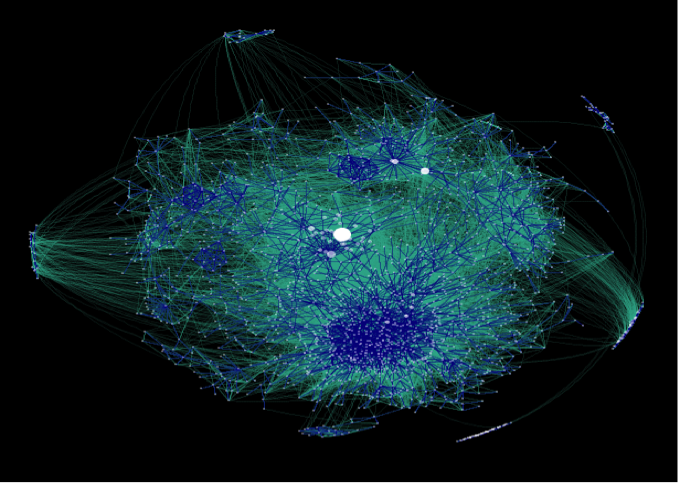
\includegraphics[width=15cm]{blog.png}
  \caption{Blogosphere as social network \cite{hurst2007}}
  \label{Figure:figex2a}
\end{figure}

\subsection{Social Networking Services}

In 2003, one of the earlier social networking website Friendster \footnote{\url{www.friendster.com/}} had attracted 5 million users that created profile and connected with friends and family, soon many other similar website emerged of which Facebook was the most successful with more than 900 million user as of March 2012. People create explicit connect with friends or colleagues (LinkedIn) to communicate and share contents with them.

People use these websites in every aspect of their life, they use it to share personal information with friends and family, use it to share their work and interest with colleagues and play games with other users. Now, business enterprise have also adopted these social networking website to connect to their consumers and advertise the products directly to the people who are interested in it \cite{ridings2004virtual}.

These websites now, not only connect people together through personal connection, it also connects people through shared objects. A good example of this is Facebook 'Like' button, this is used to connect people who like the same music or movies or share similar interest. This creates a vast community of people who share same interest and also share similar information. This giant global graph of people and object connected together is similar to the idea of Linked Data.

\subsection{Microblogging}

There are also microblogging services like Twitter and Tumblr \footnote{\url{https://www.tumblr.com/}}  makes sharing information quicker and faster. These services create implicit relationship between people by follower-following method. The social network grows quickly as people do not need to approve any friendship and the content is distributed widely and rapidly by the re-sharing feature they have. Users can retweet the same tweet in Twitter and reblog the same posts in Tumblr multiple times creating a viral distribution of information.

There are more than 500 million twitter users as on April 2012 and there are 400 million tweets everyday. Analysis of the tweets has suggested that 40\% of the tweets are pointless babbles and only 13\% have some value or important information or news \cite{Whitelaw2011}. The rest of the tweets are spams, conversations or self-promotion and marketing. Twitter and Tumblr allow users to interact, create hash tags and share pictures, videos and other media.

\subsection{Peer to Peer network}

The other method of collaborative information sharing is peer-to-peer network where peers are the computers system connected through Internet. Some software applications like Bit Torrent \footnote{\url{www.bittorrent.com/}}  are used to share any content between the users and large documents can easily be shared by reducing the load on one server. There are many controversy and legal issue with sharing copyright files like music, films and books but this social network allows millions of people to share large amount of data in distributed format.

\subsection{Content Specific Social Networking services}

After Facebook, a new trend emerged for content specific social networking websites like YouTube to watch videos, Flickr to share pictures, Delicious \footnote{\url{http://delicious.com/}}  to share bookmarks, LastFM \footnote{\url{http://www.last.fm/}}  to listen to music, etc. In these websites people connect with other people with similar interest and passion. They form groups and communities and use user participation rate the content for quality control and user behaviour recommendation.

These are open networks where people can upload their content and it is visible to the whole world. It gives a platform to broadcast creative content to the large audience. These networks are completely depended on user contribution to sustain the community.

\section{Collective Intelligence and Crowdsourcing}

The World Wide Web provided a platform for people to share, discuss ideas and information, and collaborate with each other. The Web 2.0 main trend was using the collective intelligence of people to create a knowledgebase, get user preference and do recommendations.

\subsection{Wiki}

Web 2.0 provided easy to use tools for collaborative authoring and ownership of information. A wiki allows users to add, remove, edit or modify any content on a webpage and keep tracks of different versions changes. Wikipedia \footnote{\url{http://www.wikipedia.org/}}, a collaborative encyclopaedia, is an excellent example where people with similar interest and expertise came together to create this vast knowledgebase. Crowdsourcing is used for quality control and to stop vandalism spamming. These collaborative networks strive because they enforce a strong sense of community with people through collaboration and creation of content where individual contribution was counted and it became an efficient knowledge management tool.

\subsection{Folksonomy}

The other feature of Web 2.0 was the ability to add tags to any content and user generated taxonomy is utilized to categorize the pictures, videos, music and every kind of data. The tags make sit easier to classify and categorize information and also to search and discover similar content on any topic. Collaborative tagging and bookmarking is used to add metadata and categories to pictures in Flickr and links in Delicious and it makes it easier for people to search and discover information. Using multiple tags also connects categories and geo-tagging helps in identifying any object based on location.

\subsection{Open Source Software}

Linux open source software project gave an alternative to the traditional software development and the programmers formed a community to build the software and tools. The system provided the developers with a platform to collaborate and create where individual authorship is recognized but they don�t get exclusive intellectual rights. Creative common license is used and it allows the creator to easily mark their creative work and share it with the world.

This type of large-scale software development requires lots of co-ordination and communication with the community and a project is divided into various phases of development. There are many tools available, like version control, bug tracking, task management and testing tools, for people to collaborate and communicate. Many software products like Firefox, Android, etc. are successfully developed and used by general mass.

\subsection{Forums and messaging boards}

Forums and boards gave a place for people to meet anonymously and have a discussion, it was the beginning of virtual community where face to face communication was replaced by messaging boards, chat rooms, question and answer forums. These online communities were formed based on interest and common objective and people from all around the world could come together and communicate on a particular topic of interest \cite{adamic2008knowledge}.

\subsection{User Recommendation system}

The power of collective behaviour and knowledge was utilized by the websites like Amazon \footnote{\url{http://www.amazon.com/}} and Pandora \footnote{\url{www.pandora.com/}} for recommendations of books and music respectively. Users in these websites also rate and review the things and crowdsourcing is used for predicting users� needs and contents can be recommended accordingly.

\subsection{Human Computation}

Humans are good at solving the AI complete problems like natural language processing, image analysis that computers still have problem solving. Luis von Ahn came up with various systems to utilize human computation and use crowdsourcing to solve these problems. The ESP games \cite{vonAhn2004} are used to annotate images on the web \cite{von2006games}, reCaptcha \cite{vonAhn2003} is used to digitize millions of book and Duolingo \footnote{\url{http://duolingo.com/}} is used to translate the web into various languages.

These systems are used by users to play games, identify humans from machines to stop spams, and to learn foreign language and they utilize the tasks easily done by human to solve computational problems. The same task done by many people give a common consensus to knowledge and prevent errors \cite{von2009human}.

\section{Semantic Web and Social Networking}

The idea of a Semantic Web was coined by sir Tim Berners-Lee in his Scientific American article \cite{berners2001semantic} that described it as an extension of the current web, where all data is structured and has a meaning accessible by both machines and people. Linked Data is a set of best practices for publishing reusable structured contents using the existent Web as a sustaining framework. In Linked Data every resource is represented by a URI and HTTP URIs are used in order to retrieve documents that describe those resources. Documents are described with RDF where links to other resources are then used.

There are many Semantic Web technologies and application available in the area of social network and social media. These technologies help with data representation, data portability and cross platform interoperability. Using Linked Data principles a decentralized system can be created that helps in social network integration. Every object and entity is identified using a URIs and it is deferenceable by using HTTP \cite{shadbolt2006semantic}. Also, useful metadata about the entities can be added in structured format using RDF and it could be linked with other related data to improve discovery. Some of the social semantic technologies and application is discussed below.

\subsection{Social Semantic Technology}

As previously discussed there is already a large amount of linked data available on Web called Open Linked Data cloud and there are many useful ontologies to represent this data, including social data. The evolution and formation of different and most widely used ontologies to describe people, communities, and their data are discussed below.

\subsubsection{FOAF}

FOAF ontology is used to describe people and the relationship between them. Each person has a unique identifier and a specific vocabulary is used to create personal profile of the users and describe their social network. It can be easily integrated with other Semantic Web ontologies and a person can describe one or more of their online social network \cite{brickley2010foaf}.

Many websites like LiveJournal, FriendFeed, identi.ca uses FOAF to describe their users. Many other websites has plug-in or external application that create their FOAF profile like FOAF generator, WordPress plug-in etc. It helps to solve distributed identity problem when one user has different account in different website, using FOAF, a user can combine all the information from various sources into one file and interlink his different identity and social network. This also helps in creating a complete user profile and cross-site content recommendation \cite{bojars2008interlinking}.

Privacy and digital identity protection issues can also be resolved in FOAF by using SSL protocol that provides distributed authentication system to different user and create different policy for private and public information \cite{bojars2008weaving}.

\begin{figure}[!htb]
  \centering
  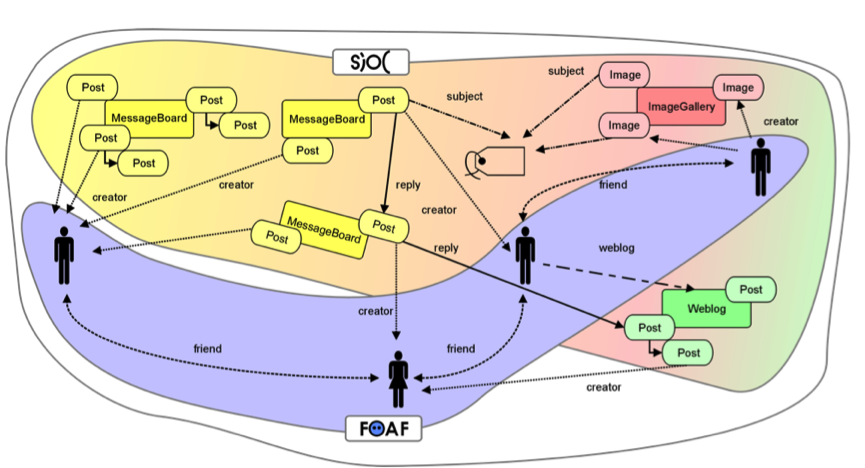
\includegraphics[width=15cm]{foaf.png}
  \caption{Creating a FOAF profile and SIOC file of a user.}
  \label{Figure:figex2b}
\end{figure}

\subsubsection{SIOC}

SIOC ontology is used to describe online communities� activities and interlink them together. It can be easily integrated with FOAF profile of a user, so the combined document contains users� information, their social network and all the data user created with the comments and metadata provided by others \cite{breslin2005towards}.

SIOC can be used for blogs, forums, discussion board, mailing lists, etc. Many websites uses SIOC as well as ma enterprise and E-government uses SIOC to freely available their data.

SIOC is the next step in integrating different social networks together, it describes the content of the website with a structured format so the information is easier to access, search, and discover. The posts can be browsed in many innovative ways by using specialized queries. It creates connection between people from different networks and people with different account can use it with FOAF to prevent identity problems or co-referencing. It makes it easier for people to connect the data in decentralized system ad enable data integration \cite{breslin2007future}.

The above figure describes how FOAF and SIOC together can help interlinking and integrating different communities and different account of the same person together using Semantic Web technology for easy reusability.

\subsubsection{OPO}

The OPO ontology is used to describe the online presence of a user who is using instant messaging service. It stores the state of user, if they are online or offline and who they are communication with and what they are communication.

\subsection{Social Semantic Applications}

Social web and semantic web has come a long way in past ten years. There are many social semantic application available present on the web that solves many underlying problem present in the SNS. They are described below \cite{Gruber2008}.

\subsubsection{Semantic Tagging}

People in Web 2.0 use tags to classify, categorize or group their content using their own vocabulary. This has enabled users to generate more data but this also ambiguous and imprecise.   People use different terms in the same context meaning the same concept and same terms in different contexts for different meanings.

The main issues with tags are the tag ambiguity problem where it is not clear in what context a tag is used. For example if a post tagged with �Apple� is describing a fruit or a computer brand. That�s why is so important to reconcile lexical tags to URIs that unambiguously identify the meaning of a term \cite{garcia2009preliminary}. The same tag actually differs when people use different spelling or space or hyphen between words. And there is also a lack of organization and hierarchy between tags \cite{correndo2007survey}. It is hard to comprehend if a tag marked �Apple� is a subclass of a tag marked �Fruit.�

Most of these problems can be solved by the MOAT ontology that helps to describe the meaning of a tag semantically and connect it with the object and related tags. Also the co-occurrence of tag can be used to group similar tags together. It is user defined interlinking and the contents are linked to the Linked Data Cloud. It uses the collaborative approach to share the meaning of tag in a community.

The Tag Ontology helps to solve the ontological and hierarchical problem that exists between groupings of tags. The SCOT (Social Semantic Cloud of Tags) ontology creates a model to describe a tag cloud and it makes the tag cloud portable so it can be exported from one service to another without losing the data.

Many research is carried out in the area of extracting ontologies from tags, FolksOntology is one of those project that extracts relationships between tags. FLOR is another project that automatically identifies the meaning of a tag. These ontologies can be combined with other ontologies to create a complete model for semantic tagging in the area of social network \cite{bojars2008interlinking}.

\subsubsection{Semantic blogging and microblogging}

Blogosphere is a huge part of the web where people are generating data in exponential rate, but most of this data is not structured or categorized, it is in plain text \cite{chin2006social}. With the advent of Twitter, microblogging is the new trend and this also lacks context and structure.

Semantic web technologies can be used to semantically annotate useful content and keywords of the blog posts and micro blogs to add meaning and structure to it. Drupal \footnote{\url{http://drupal.org/}} website provides an easy to use platform to add annotation to the blog posts and it embeds RDFa into them. Twitter Annotation service takes the tweet metadata of location, time, etc. and annotates them to provide semantic metadata.

Another important project that helps in semantic blogging is the Open Graph Project and Facebook Open Graph that helps users to express preferences increasing in this way the quality of the information provided in the blogs or indeed in any website \cite{rowe2009interlinking}. People can add reviews and ratings to a movie or use the Facebook �Like� button to show their preference and the Open Graph project connects the objects and resources with people, their friends and people with similar interest to provide better recommendation. These projects follow an Open Graph Protocol and create the data in RDF and the data can be queried to provide useful information.

The main use of these technologies is that it is easier for users to publish their data in structured format and they can publish it cross-site because it is portable. The developers can quickly create mash-ups to provide better data visualizations by integrating data from different sites because search and discover is easy in structured data. This data can also be mapped to people�s FOAF profile and SIOC data files. If the dataset has a SPARQL endpoint, querying and retrieval of data can be done \cite{millard2010consuming}.

\subsubsection{Semantic Wiki}

Wiki is an excellent example of collaborative creation and edition for emergent knowledge. There is a large number of people editing Wiki pages and helping in maintaining the quality of the information and preventing spam and irrelevant information \cite{chi2009augmented}. The structured information from the Wikipedia info-boxes has already been converted into linked data within the DBpedia \footnote{\url{http://dbpedia.org/}} project, and this data set is already one of the largest and most linked dataset in the Open Linked Data cloud.

DBpedia is very useful because it uses Wikipedia data and it is easy for anyone to read or write a Wikipedia article, and it also solves the problem machines cannot by using Crowdsourcing. But DBpedia only uses part of the data because Wikipedia lacks proper structure and agreed semantics of the data and its categories. This problem can be solved by semantic wiki where all the data is structured and properly categorized. This provides better search and discovery of information like in OntoWiki \cite{Albors2008}.